\documentclass[danish,a4paper,twocolumn,amsmath,amssymb]{revtex4-1}
\usepackage{babel}		%Giver mulighed for dansk orddeling. Slet kun hvis du VED hvad du laver, eller skal skrive noget på engelsk.
\usepackage[latin1]{inputenc}	%Tillader danske tegn
\usepackage[T1]{fontenc}	%Tillader danske tegn
\usepackage{graphicx}		%Tillader indsættelse af billeder
\usepackage{dcolumn}		%Bruges til at lave matematiske tabelsøjler... se datatabel
\usepackage{booktabs}		%linjer i tabeller...
\usepackage{mathtools}		%Ekstra matematik... bare lad den være, du får muligvis brug for den.
\usepackage{multirow}
\usepackage{threeparttable} 			% Jeg kan ikke huske hvad den gør, men den skal bruges til for at tabelnoterne virker
\usepackage[tableposition=top]{caption} % Noget med at lave caption så det står godt
\usepackage[version=3]{mhchem}  %\ce{H2O + e^{-} -> H2O^{+} + 2e^-}
%siunitx-pakken er ny ift. den originale template, så der henvises i tekstan til en anden pakke, beklager.
\usepackage{siunitx}	%Bruges \SI{<tal>}{<enhed>}, \si{<enhed>} eller \num{<tal>}.
\sisetup{output-decimal-marker={,},separate-uncertainty=true}%Sørger for komma som decimalmarkør. Virker også ved decimaltal, hvis man bruger \num{<tal>}.
\usepackage{url}		 %bruges til at formattere url'er... kan sagtens udelades.
%Det følgende laver to makroer, \tref{} og \fref, der kan bruges ligesom \ref til at referere til hhv. tabeller og figurer. 
%De indsætter selv ordet Tabel/Figur, og sørger for at der ikke sker et linjebrud mellem dette og nummeret.
\newcommand{\tref}[1]{\tablename~\ref{#1}}
\newcommand{\fref}[1]{\figurename~\ref{#1}}
%Tilsvarende for ligninger. Indsætter "ligning (#)".
\newcommand{\lref}[1]{ligning~\eqref{#1}}
	% \eqref laver en reference med parenteser omkring (til brug ved ligninger.)

%Disse makroer indsætter ordene "PicoScope" og "EasyPlot" i teksten (med store bogstaver. Husk at sætte "{}" bagefter for at få et mellemrum.
%Jeg har lavet dem fordi jeg blev træt af at sidde og trykke shift hele tiden, og for at få det til at stå ens. Brug dem, eller lad være.
\newcommand{\picos}[0]{\textsc{PicoScope}} %hedder \picos for ikke at komme i kambolage med pico fra SIunits.
\newcommand{\epw}[0]{\textsc{EasyPlot}}    %epw er navnet på programfilen for easyplot, men det har ingen betydning for makroen. Jeg valgte det fordi det var noget jeg kunne huske, og det kan sagtens ændres.
\newcommand{\matl}[0]{\textsc{Matlab}} %Skriver Matlab med small caps.
\usepackage[footnote,draft,english,silent,nomargin]{fixme}
%hyperref-pakken kan bruges til at redigere pdf-metadata. Det kan være et nice touch, men er generelt ikke påkrævet. Laver automatisk referencer i teksten til farvede hyperlinks i.
\usepackage{hyperref}
\hypersetup
{   pdfsubject={Rapport},
	pdfauthor={Alexander Rasborg Knudsen}
    pdftitle={Masse},
    pdfstartview=FitH,
    colorlinks=true}
    
%Følgende gør, at subscripts bliver ikke-kursiv. Anvendes X_|<subscript>|. Erstattes evt. med X_{\mathrm{<subscript>}}.
\makeatletter
\begingroup
\catcode`\_=\active
\protected\gdef_{\@ifnextchar|\subtextup\sb}
\endgroup
\def\subtextup|#1|{\sb{\textup{#1}}}
\AtBeginDocument{\catcode`\_=12 \mathcode`\_=32768 }
\makeatother

\usepackage[danish=quotes]{csquotes} %Danske citationstegn. \enquote{}

%Lad disse to linjer være. De sørger for at bunden af siden bliver pæn, og fjerner indryk ved afsnit.
\raggedbottom
\parindent = 0pt




\begin{document}
\title{TINON Project: Speaker recognition}

\author{Kasper Nielsen}%Forfatter 1
\author{Alexander Rasborg Knudsen}%Forfatter 2
\affiliation{Department of Engineering, Aarhus Universitet} 
\date{\today} %Dato.

\begin{abstract}
\bigskip

\end{abstract}

\maketitle
\noindent

%!TEX root = Main.tex
\section*{Introduction}
The purpose of this case project is to take the learnings of the course \emph{Non-linear Signal Processing and Pattern Recognition (TINONS1)} and apply them to a specific signal processing or pattern recognition problem.
In this case the object is to create a speaker recognition system.
The system shall be able to recognize a specific speaker from a ensemble of speaker models.

The topics from the TINONS course that will be applied in relation to this case are:
\fxnote{List if necesary} 
		

\section*{Data Collection}

This projects dataset consist of 1.656 sound files. 
Divided into a large training set and a smaller test set. 
Each file is 2 seconds long and was recorded at 48 kHz.
The data structure consist of 4 persons stating a number between 0 to 9. 
The data is borrowed with permission from Christoffer Mose, Simon Madsen, Camilla Munk and Jacob Hansen.
  

%!TEX root = Main.tex
\subsection*{Feature Extraction}
When doing speaker recognition it is advantageous to classify on the basis of extracted features from speech data, rather than the audio samples themselves \cite{Springer:36}.
Features were extracted on a frame-to-frame basis.
This was done on the assumption of pseudo-stationarity of human speech in the scale of a few tens of ms \cite{Springer:36}.
The frames consisted of 256 samples, with a new frame staring every 100 samples.
This means that we have a frame length of
\begin{equation}
t_{frame length} = \dfrac{N_{frame}}{F_s} = \dfrac{256}{48\ kHz} = 5.33\ ms
\end{equation}

and a frame interval of
\begin{equation}
t_{frame interval} = \dfrac{N_{interval}}{F_s} = \dfrac{100}{48\ kHz} = 2.08\ ms
\end{equation}

The features extracted for use in classification were $12^{th}$ order Mel-frequency Cepstral Coefficients (MFCC), as they hava proven effective in speaker regocnition applications and speech processing in general.
Further, so-called delta and double-delta coeffcients, the temporal derivatives $ \frac{dC}{dt} $ and double-derivatives $\frac{d^2C}{dt}$ of the MFCCs respectively, are used as features.
\footnote{For more on MFCC and feature extraction, see Appendix} \fxnote{fix footnotes}

\begin{figure}[H]
\centering
\includegraphics[width=0.5\linewidth]{MFCC_Flowchart_CROP}
\caption{MFCC}
\label{fig:MFCC_Flowchart}
\end{figure}


%!TEX root = Main.tex
\section*{Classification}

%!TEX root = Main.tex
\section*{Linear Classification}
In linear classification the decision surfaces are linear functions of the input vector $\mathbf{x}$.
the target of the classification is labelled in the target variable $\mathbf{t}$, using the target values to represent class labels.
In this project there are 3 different speakers, $K = 3$ then the target vector for class 3 be $\mathbf{t} = (0, 0, 1)^T$.
The value of $t_k$ can be interpreted as the probability of the given class being class $C_k$.
To assign each vector $\mathbf{x}$ with a specific class.
The linear discriminant function in its simplest form
\begin{equation}
y(\mathbf{x}) = \mathbf{w}^T \mathbf{x}+w_0
\label{eq:lin_output}
\end{equation}

\paragraph*{Training}
The linear classifier is applied to the training dataset, containing feature vectors $(\mathbf{x}_n)$ and the target vectors $(\mathbf{t}_n)$.
The vectors are on the form:
\begin{equation}
\mathbf{\tilde{X}}=\left[ \begin{array}{c}\mathbf{x}_1^T \quad 1\\
\mathbf{x}_2^T \quad 1\\
...\\ 
\mathbf{x}_n^T \quad 1 \end{array} \right],
\;
\mathbf{T}=\left[ \begin{array}{c}
\mathbf{t}_1^T\\ 
\mathbf{t}_2^T\\ 
...\\
\mathbf{t}_n^T
\end{array} \right]
\label{eq:linearVectors}  
\end{equation} 

This calculation are done to determine the $\tilde{\mathbf{W}}$:
\begin{equation}
\tilde{\mathbf{W}} = \tilde{\mathbf{X}}^\dagger \mathbf{T} \approx  (\tilde{\mathbf{X}}^T \tilde{\mathbf{X}}+\mathbf{I})^{-1} \tilde{\mathbf{X}}^T\mathbf{T}
\label{eq:weightVector}  
\end{equation}
The resulting parameter matrix W ̃ was tested using the test set.
\paragraph*{Result}
The result of the linear classifier is a total accuracy of 55.9, 51.2 and 50.6 \% respectively for one, two and ten digits. 


\subsection*{Dimensionality Reduction}

\begin{figure}[H]
\centering
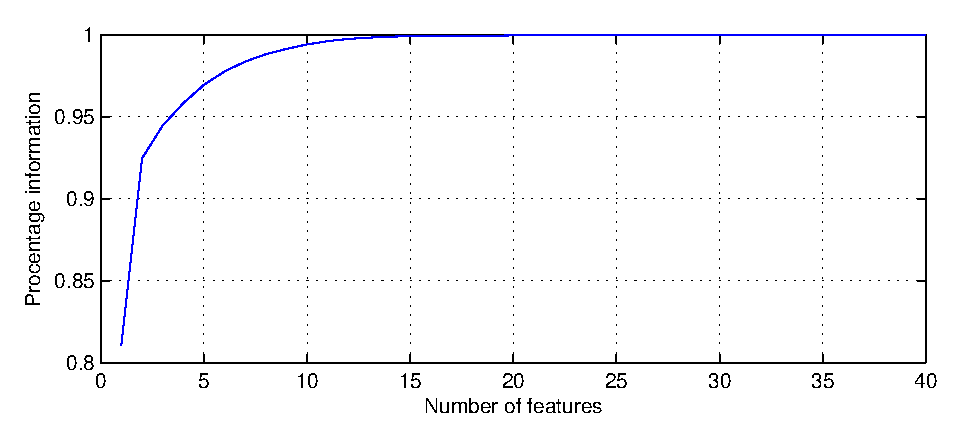
\includegraphics[width=\linewidth]{PCA_dist_var}
\caption{Cumulative distribution of variance (information) in dimensions sorted by highest eigenvalue}
\label{fig:PCA_dist_rap}
\end{figure}

%!TEX root = Main.tex
\section*{Gaussian Mixture Models}
Gaussian Mixture Models (GMM) is a way of finding and describing sub-populations in clusters of data points.
It is done by fitting a specified number of Gaussian distributions to a population of data points.
Each distribution is a component of the model. 
The individual data points are then arranged into clusters based on which model component is most likely given the observed data point.

The distributions of the mixture model are fitted to data by iteratively employing Expectation Maximization (EM).

\subsection*{The EM Algotrithm}
In EM a mixture model is iteratively updated by esitimating model parameters $\bm{\mu}_k $ (component means) and $ \bm{\Sigma}_k $ (component covariance matrix) based on current assignment of responability and then reassigning responability based on new model parameters, starting out with a random guess of $\bm{\mu}_k \text{ and } \bm{\Sigma}_k \text{ for } k=1..K$ 


\subsubsection*{Initialization:}
\begin{enumerate}
\item
Choose initial estimates for model parameters $ \mathbf{\pi}_{k}, \mathbf{\mu}_{k}, \mathbf{\Sigma}_{k} $.

\begin{itemize}

	\item
	$ k $ is the component number out of K.

	\item
	$ \pi_{k} $  is the weight of the \textit{k}th component.

	\item
	$ \mathbf{\mu}_{k}$ is the mean of the \textit{k}th component.

	\item
	$ \mathbf{\Sigma}_{k} $ is the covariance matrix of the \textit{k}th component.

	\end{itemize}


\item
Compute the initial log-likelihood og the model

\begin{equation} \label{eq:loglikeGMM}
\ln p\left(X | \mathbf{\mu}, \mathbf{\Sigma}, \pi\right) = 
\sum_{n=1}^{N} \ln \sum_{k=1}^{N} \pi_{k}\mathcal{N}(\mathbf{x}_{n}|\mathbf{\mu}_{k},\mathbf{\Sigma}_{k})
\end{equation}

\end{enumerate}

\subsubsection*{E-step:}
Calculate the probability of each point in each component in order to assing responsibility

\begin{equation}
\gamma_{nk} = 
\frac
{\pi_{k}\mathcal{N}(\mathbf{x}_{n}|\mathbf{\mu}_{k},\mathbf{\Sigma}_{k})}
{\sum_{j=1}^{K} \pi_{n}\mathcal{N}(\mathbf{x}_{n}|\mu_{j},\mathbf{\Sigma}_{j})}
\end{equation}

\subsubsection*{M-step:}
Estimate new guesses for $ \mathbf{\pi}_{k}, \mathbf{\mu}_{k}, \mathbf{\Sigma}_{k} $.

\begin{equation}
\mathbf{\mu}_{k}^{new} = 
\frac{1}{N_{k}}
\sum_{n=1}^{N} 
\gamma_{nk}
\mathbf{x}_{k}
\end{equation}

\begin{equation}
\mu_{k}^{new} = 
\frac{1}{N_{k}}
\sum_{n=1}^{N} 
\gamma_{nk}
(\mathbf{x}_{k} - \mathbf{\mu}_{k}^{new})
(\mathbf{x}_{k} - \mathbf{\mu}_{k}^{new})^{T}
\end{equation}

\begin{equation}
\pi_{k}^{new} =
\frac
{N_{k}}
{N}
\end{equation}

\subsubsection*{Convergence check:}

Recalculate log likelihood using Equation \ref{eq:loglikeGMM}.
If the log likelihood has not changed more than some predetermined threshold stop iteration.
Otherwise continue from E-step.

\paragraph*{Training}
GMM is a tyoe of unsupervised machine learning, and is a first hand not usefull in our project, but by training a GMM for each speaker based on the pre-classfied trainging set, you end up with a very effective model.


Then, for each speaker, a GMM is fitted to the respective speakers' training data, using MATLAB's Statistics Toolbox.

\paragraph*{Result}


\input{MultiLayerPerceptron}

\bibliographystyle{ieeetr}
\renewcommand{\bibname}{2 Reference Document}
\addcontentsline{toc}{chapter}{2 Reference Document}
\bibliography{10731@post.au.dk-RefList}



\end{document}
